\section{Umsetzung}
\subsection{Überblick}
Genau wie bei Bitcoin besteht die Möglichkeit die Glücksspielanwendung entweder mithilfe eines ''Light Nodes'' direkt, oder über einen ''Full Node'' indirekt mit dem Ethereum Netzwerk kommunizieren zu lassen. Für den Ethereum Teil dieser Masterarbeit findet die Kommunikation indirekt über einen Full Node statt. Dies ist in Abbildung \ref{fig:anwendung_aufbau} verdeutlicht. Der Full Node empfängt Transaktionen und Blöcke, validiert diese und akualisiert kontinuierlich den Zusatnd der durch die Transaktionen veränderten Ethereum Accounts. Über die RPC Schnittstelle stellt er diese Daten nach außen bereit. Die Java Bibliothek Web3J \cite{web3j} erleichtert den Aufruf der RPC Schnittstelle des Full Nodes. Anders als bei Bitcoin benötigt die Glücksspielanwendung keine eigene Datenbank, da der Zustand des aktuellen Topfs im Smart Contracts und somit ''in der Blockchain'' gespeichert ist.
\begin{figure}[H]
\centering
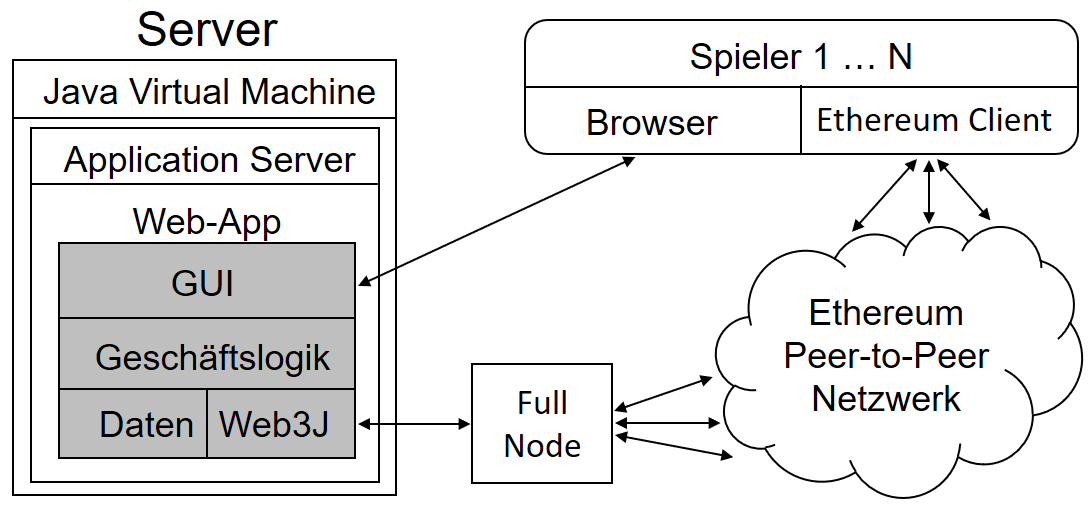
\includegraphics[width=1\linewidth]{Figures/umsetzung_eth/anwendung_aufbau}
\decoRule
\caption{Ethereum: Netzwerk Integration}
\label{fig:anwendung_aufbau}
\end{figure}

Möchte man eine Anwendung direkt in das Ethereum Netzwerk integrieren, bietet sich in Java die Bibliothek EthereumJ \cite{ethereumj} an. 

\subsection{Smart Contract}
Die folgenden Codestücke beschreiben den TrustlessGambling Smart Contracts in der Sprache Solidity\footnote{\url{https://solidity.readthedocs.io/en/v0.4.0/}}.

\subsubsection{Datenmodell}
Das folgenden Codestücke zeigt den Rahmen, alle Variablen und den Konstruktor des Smart Contracts.
\begin{lstlisting}[basicstyle=\small]
pragma solidity ^0.4.0;
contract TrustlessGambling {
    // constants
    uint8 public constant NBR_OF_SLOTS =3;
    uint public constant EXPECTED_POT_AMOUNT=1000;// WEI
    uint8 public constant PAYOUT_BLOCK_OFFSET =1;    
    // pot values
    uint public nbrOfParticipants;
    address[NBR_OF_SLOTS] public depositAddresses;
    address[NBR_OF_SLOTS] public payoutAddresses;
    uint public closingBlockNumber;
    uint public payoutBlockNumber;
    bytes32 public payoutBlockHash;
    uint public winner; // 0 -> NBR_OF_SLOTS-1
    bool public potClosed;
    uint public nbrOfMissedPayouts;
    // constructor
    function TrustlessGambling() public {
        nbrOfParticipants = 0;
        potClosed = false;
        nbrOfMissedPayouts = 0;
    }
}
\end{lstlisting}


Zeile 1 definiert in welcher Version der Solidity Sprache der Smart Contract geschrieben ist. Dies muss vom Compiler berücksichtigt werden. Zeile 2 legt den Namen des Smart Contracts fest. Über die beiden Konstanten in Zeile 4 und 5 kann man die Anzahl Spieler, und den von jedem Spieler erwarteten Einzahlungsbetrag festlegen. Die in Zeile 6 festgelegte Konstante legt fest, welcher Block ab der letzten Einzahlungstransaktion den Gewinner festlegt. Diese Werte können nach der Bereitstellung des Smart Contracts nicht mehr verändert werden. Die Variablen von Zeile 8 bis Zeile 16 werden vom Smart Contract manipuliert und speichern den Zustand des aktuellen Topfes. Zeile 8 speichert wie viele Teilnehmer bereits eingezahlt haben. Zeile 9 und 10 speichern die Ein- und Auszahlungsadressen der aktuellen Teilnehmer. Die Zeilen 11 bis 14 speichern alle für die Gewinnerauswahl benötigten Werte. Zeile 15 definiert über den Wahrheitswert \code{potClosed}, ob der Topf offen ist und Einzahlungen stattfinden können, oder ob der Topf geschlossen ist. Der Nutzen des Wertes aus Zeile 16 wird in Abschnitt \ref{sssec:eth_nbrOfMissedPayouts} erklärt. Zeile 18 bis 22 beinhalten den einmalig bei der Bereitstellung des Smart Contracts aufgerufenen Konstruktor. Alle Variablen des Smart Contracts sind zur Schaffung maximaler Transparenz mit dem Schlüsselwort \code{public} markiert. Dies erlaubt es den Nutzern, alle Werte des Smart Contract abzurufen.

\subsubsection{Einzahlungen}
Einzahlungen finden über die beiden \code{deposit} Methoden statt. Diese sind mit dem Schlüsselwort \code{payable} markiert. Dies bedeutet, dass Transaktionen einen Ether-Betrag beim aufruf dieser Methoden angeben können.
\begin{lstlisting}
function deposit() payable public {
    deposit(msg.sender);
}
function deposit(address _payout) payable public {
    assert(msg.value == EXPECTED_POT_AMOUNT);
    assert(!potClosed);
    depositAddresses[nbrOfParticipants] = msg.sender;
    payoutAddresses[nbrOfParticipants] = _payout;
    nbrOfParticipants++;
    if (nbrOfParticipants == NBR_OF_SLOTS){
        closingBlockNumber = block.number;
        payoutBlockNumber = closingBlockNumber + PAYOUT_BLOCK_OFFSET;
        potClosed = true;
    }
}
\end{lstlisting}


Nutzt der Spieler die Methode aus Zeile 1, wir als Auszahlungsadresse einfach die Adresse der Transaktion verwendet. Nutzt der Spieler die Methode aus Zeile 4, hat er die Möglichkeit eine beliebige Auszahlungsadresse anzugeben. Bei der Einzahlung wird zunächst in Zeile 5 geprüft, ob der der Topf offen ist. Ist dies der Fall, prüft Zeile 6, dass der Eingezahlte Betrag mit dem fest definierten Wert übereinstimmt. Anschließen werden die Ein- und Auszahlungsadresse abgespeichert und die aktuelle Anzahl Teilnehmer um eins erhöht. Zeile 10 prüft, ob es sich um die letzte Einzahlungstransaktion handelt und schließt den Topf gegebenenfalls. Bevor der Topf geschlossen wird, wird allerdings noch in Zeile 11 die aktuelle Blocknummer abgespeichert und anschließend die Blocknummer für die Gewinnerauswahl berechnet.

\subsubsection{Auszahlungen}\label{sssec:eth_nbrOfMissedPayouts}
Auszahlungen finden durch den Aufruf der \code{payout} Methoden statt. Diese ist nicht mit dem Schlüsselwort \code{payable} markiert und erwartet keinen Ether-Betrag beim Aufruf.
\begin{lstlisting}[basicstyle=\small]
function payout() public{
    assert(potClosed);
    assert(block.number>payoutBlockNumber);
    payoutBlockHash = block.blockhash(payoutBlockNumber); 
    if(payoutBlockHash == 0){
        nbrOfMissedPayouts++;
    }else{
        winner = uint256(payoutBlockHash) % NBR_OF_SLOTS;
        address winnerAddress = payoutAddresses[winner];
        uint amount= EXPECTED_POT_AMOUNT*NBR_OF_SLOTS;
        amount += EXPECTED_POT_AMOUNT*NBR_OF_SLOTS*nbrOfMissedPayouts;
        winnerAddress.transfer(amount); // send pot amount to winner
        nbrOfMissedPayouts = 0;
    }
    potClosed = false;
    nbrOfParticipants=0;
}
\end{lstlisting}


Die Methode kann nur aufgerufen werden, falls der Topf geschlossen ist und die aktuelle Blocknummer bereits größer als die Blocknummer des Blocks für die Gewinnerauswahl ist. Sind diese Bedingungen erfüllt, hängt der weitere Verlauf der Abarbeitung der \code{payout} Methode vom Zeitpunkt des Methodenaufrufs ab. Smart Contracts können laut einer Konvention\footnote{Dies ist Effizienzgründen geschuldet. Blockheader sind in Ethereum mindestens 500 Byte groß, mit einer Blockzeit von 12 Sekunden wächst die Blockheaderkette somit täglich um 3,6 Megabyte. Der Zuwachs beträgt jährlich somit über 1 Gigabyte an Daten. Ein Ethereum Client der nicht die gesamte Blockheaderkette speichert, könnte somit nicht die Ausführung von Smart Contracts validieren, da ihm dazu die Daten aus der Vergangenheit fehlen.} bei ihrer Ausführung nur auf die Werte der 256 letzten Blockheader zugreifen\footnote{\url{http://solidity.readthedocs.io/en/develop/units-and-global-variables.html}}. Ist der in Zeile 4 angefragte \code{payoutBlockHash} älter als 256 Blocks, gibt \code{block.blockhash(<number>)} den Wert 0 zurück und Fall 1 tritt ein.
\begin{enumerate}
\item Fall: Der Aufruf der \code{payout} Methode findet zu spät statt. Es findet keine Auszahlung statt, da der Smart Contract nicht auf den entscheidenden Blockhash zugreifen kann. Der Smart Contract erhöht die \code{nbrOfMissedPayouts} Variable um eins. Dies führt dazu, dass Betrag des Topfs in den nächsten Topf verschoben wird. 
\item Fall: Der Aufruf der \code{payout} Methode findet rechtzeitig statt. Der Smart Contract berechnet in Zeile 8 den Gewinner indem er den Blockhash in einen Integer konvertiert und diese sehr hohe Zahl modulo der Anzahl Teilnehmer rechnet. Anschließend wird der korrekte Auszahlungsbetrag berechnet und in Zeile 12 an die Auszahlungsadresse des Gewinners versandt.
\end{enumerate}
Zum Schluss wird der Topf wieder geöffnet und die Anzahl der teilnehmenden Spieler auf 0 gesetzt.

\subsection{Smart Contract Bereitstellung}
Nachdem man den Smart Contract programmiert hat, muss man ihn zu Bytecode kompilieren und anschließen in einer Transaktion an das Ethereum Netzwerk senden. Dazu kann man die von Web3J bereitgestellten Comandline Tool nutzen. Dieses Tool hilft bei der Generierung einer Wallet und erlaubt es aus dem Contract Code eine Java Klasse zu generieren. Dieser Klasse ermöglicht die Interaktion mit dem Smart Contract. 

\begin{lstlisting}[basicstyle=\small]
public void createContract() throws Exception {
  String WALLET_FILENAME = "ethereum.json";
  String WALLET_PASSWORD = "changeit";
  long GAS_LIMIT = 1000000;
  ClassLoader classLoader = getClass().getClassLoader();
  File walletFile = new File(classLoader.getResource(WALLET_FILENAME).getFile());
  Credentials credentials = WalletUtils.loadCredentials(WALLET_PASSWORD, walletFile.getAbsolutePath());
  System.out.println("Account address = " + credentials.getAddress());
  Web3j web3j = Web3j.build(new InfuraHttpService("https://rinkeby.infura.io/" + UserConfiguration.API_KEY));
  BigInteger currentGasPrice = web3j.ethGasPrice().send().getGasPrice();
  TrustlessGambling contract = TrustlessGambling.deploy(web3j, credentials, currentGasPrice, BigInteger.valueOf(GAS_LIMIT)).send();
  String status = contract.getTransactionReceipt().get().getStatus();
  if ("0x1".equals(status)) {
    String address = contract.getContractAddress();
    System.out.println("Contract address = " + address);
    System.out.println("TXN hash = " + contract.getTransactionReceipt().get().getTransactionHash());
    System.out.println("Gas used = " + contract.getTransactionReceipt().get().getGasUsed());
  } else {
    System.out.println("Smart contract could not be deployed.");
  }
}
\end{lstlisting}
Die Ausführung des oben gezeigten Java Codes führt zu der folgenden Ausgabe:

\begin{lstlisting}[basicstyle=\small]
Account address = 0x2201f3919589b519135ce977cc0906c9481069b2
Contract address = 0x25c3136145fbd7f3b9217e58e2fabe3eb1928705
TXN hash = 0x06dce3c460b4caa595c5cc0f81ac78e7c70eeb1e89d3e0e6a017ea88e60dbce1
Gas used = 825846
\end{lstlisting}

In einem Blockchain Explorer kann man die Details der vom Full Node erstellten Transaktion\footnote{\url{https://rinkeby.etherscan.io/tx/0x06dce3c460b4caa595c5cc0f81ac78e7c70eeb1e89d3e0e6a017ea88e60dbce1}} und den kompilierten Contract Code\footnote{\url{https://rinkeby.etherscan.io/address/0x25c3136145fbd7f3b9217e58e2fabe3eb1928705\#code}} anschauen.
Alternativ zu Web3J lässt sich der Contract Code mithilfe eines Online Compilers \footnote{\url{https://ethereum.github.io/browser-solidity}} kompilieren und mithilfe des Ethereum Clients namens Mist\footnote{\url{https://github.com/ethereum/mist}} veröffentlichen.

\subsection{Geschäftslogik Webanwendung}

Dieses Kapitel zeigt, wie man in Etherem über einen Full Node mit dem Netzwerk interagieren kann. Die Webanwendung zeigt lediglich den aktuellen Zustand des Smart Contracts an. Die gesamte Geschäftslogik des Smart Contracts wird vom Etherem Netzwerk ausgeführt. Sollte die Webanwendung aufgrund technischer Fehler ausfallen, hat dies keinerlei Auswirkung auf das eigentliche Spiel.

TODO 

\iffalse
\begin{enumerate}
\item Es gibt sowohl test als auch mainnet. Unterscheiden sih nur leicht durch protokoll und port. Teil sehen adressen anders aus. Bei ethereum creiert man sich ein wallet und die adresse ist für beide netzwerke gültig.
\item Auf dem testents gibts faucts für entwickler, die einem ein wenig testnet cryptowährung überweisen nachdem man ein captcha gelöst hat. Problem öffters mal down.
\item Bei ethereum hatte ich das typische Java problem, dass die web3jlib eine neuere verion vewendete als der Jboss Wildfly. Daher musste ich den jboss hochziehen
\item Neuer wildfly benutzt port /127.0.0.1:9990 den auch ein nvidea network service verwendet. den musste ich dann erst abschiessen.
\end{enumerate}
\fi

\subsection{Grafische Benutzeroberfläche}

Das folgende Beispiel betrachtet einen frisch auf dem Ethereum Rinkeby Testnetzwerk bereitgestellten Smart Contract.


\begin{figure}[H]
\centering
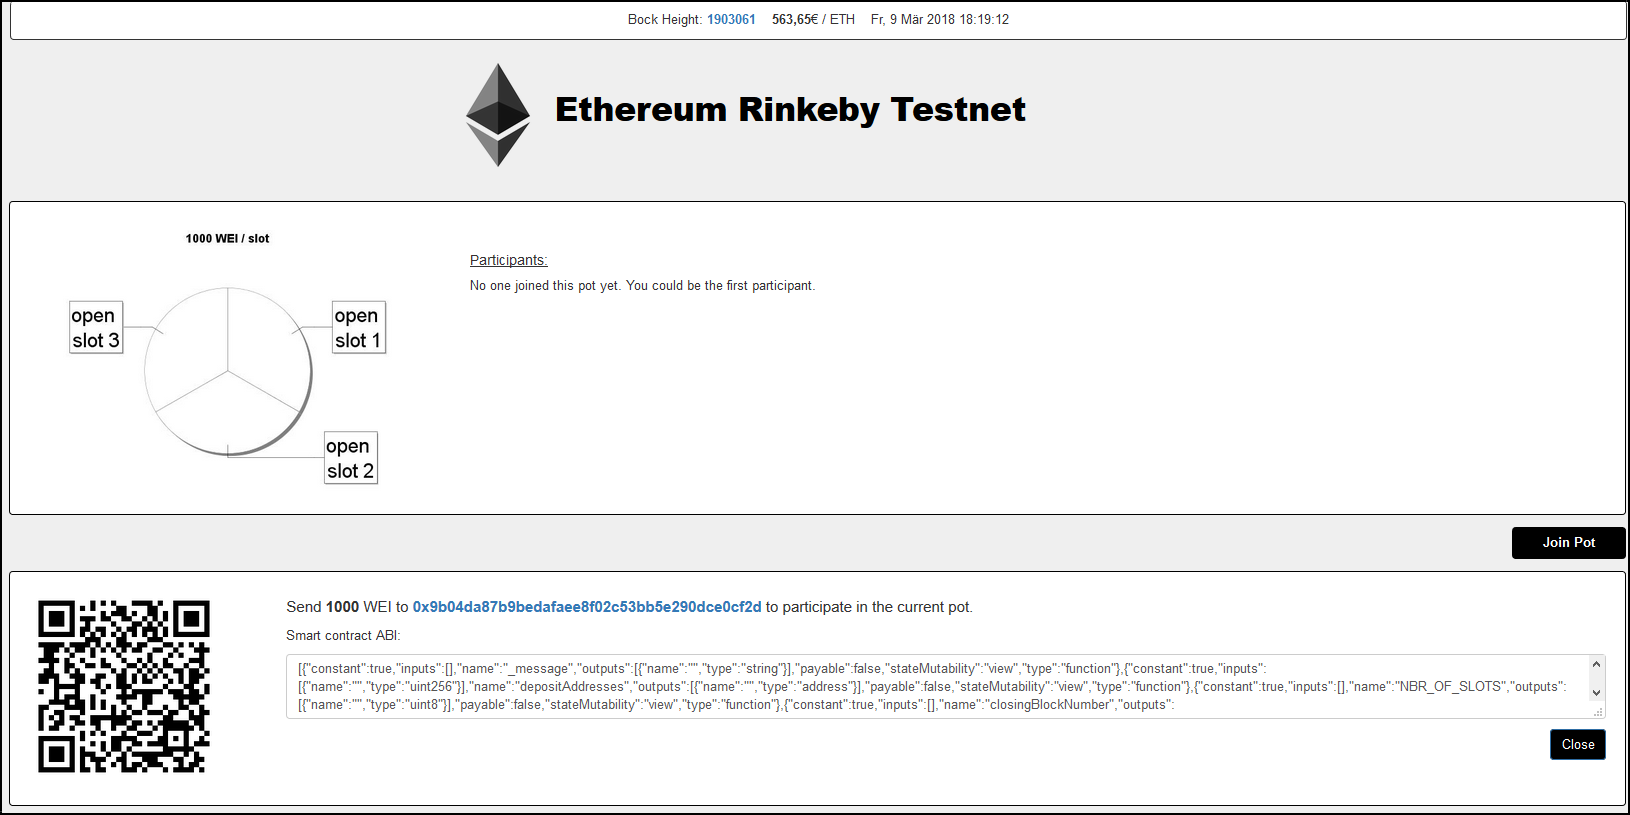
\includegraphics[width=1\linewidth]{Figures/eth_gui/ETH_pot_empty}
\decoRule
\caption{Leerer Topf}
\label{fig:ETH_pot_empty}
\end{figure}
Abbildung \ref{fig:ETH_pot_empty} zeigt einen Topf mit 3 freien Plätzen. Um dem Spiel beizutreten, muss der Spieler den Betrag von 1000 WEI (kleinste Ether Einheit) an den Smart Contract senden. Genau wie bei Bitcoin wird dem Nutzer ein QR-Code angezeigt, der die Übermittlung der Daten in einen Smartphone Client erleichtert. Das \textbf{E}thereum \textbf{I}mprovement \textbf{P}roposal Nummer 681\citep{eip21} legt die Kodierung der Daten fest.
Folgende Daten sind in dem QR Code enthalten:\\ ''ethereum:0x9b04da87b9bedafaee8f02c53bb5e290dce0cf2d/deposit?value=1000''. In diesem Beispiel verwenden wir für die Interaktion mit dem Netzwerk keinen Smartphone Client sondern die Webanwendung namens ''My Ether Wallet''\footnote{\url{https://www.myetherwallet.com/\#contracts}}. Diese benötigt für die Interaktion mit dem Smart Contract sowohl die Contract Adresse als auch das \textbf{A}pplication \textbf{B}inary \textbf{I}nterface.


\begin{figure}[H]
\centering
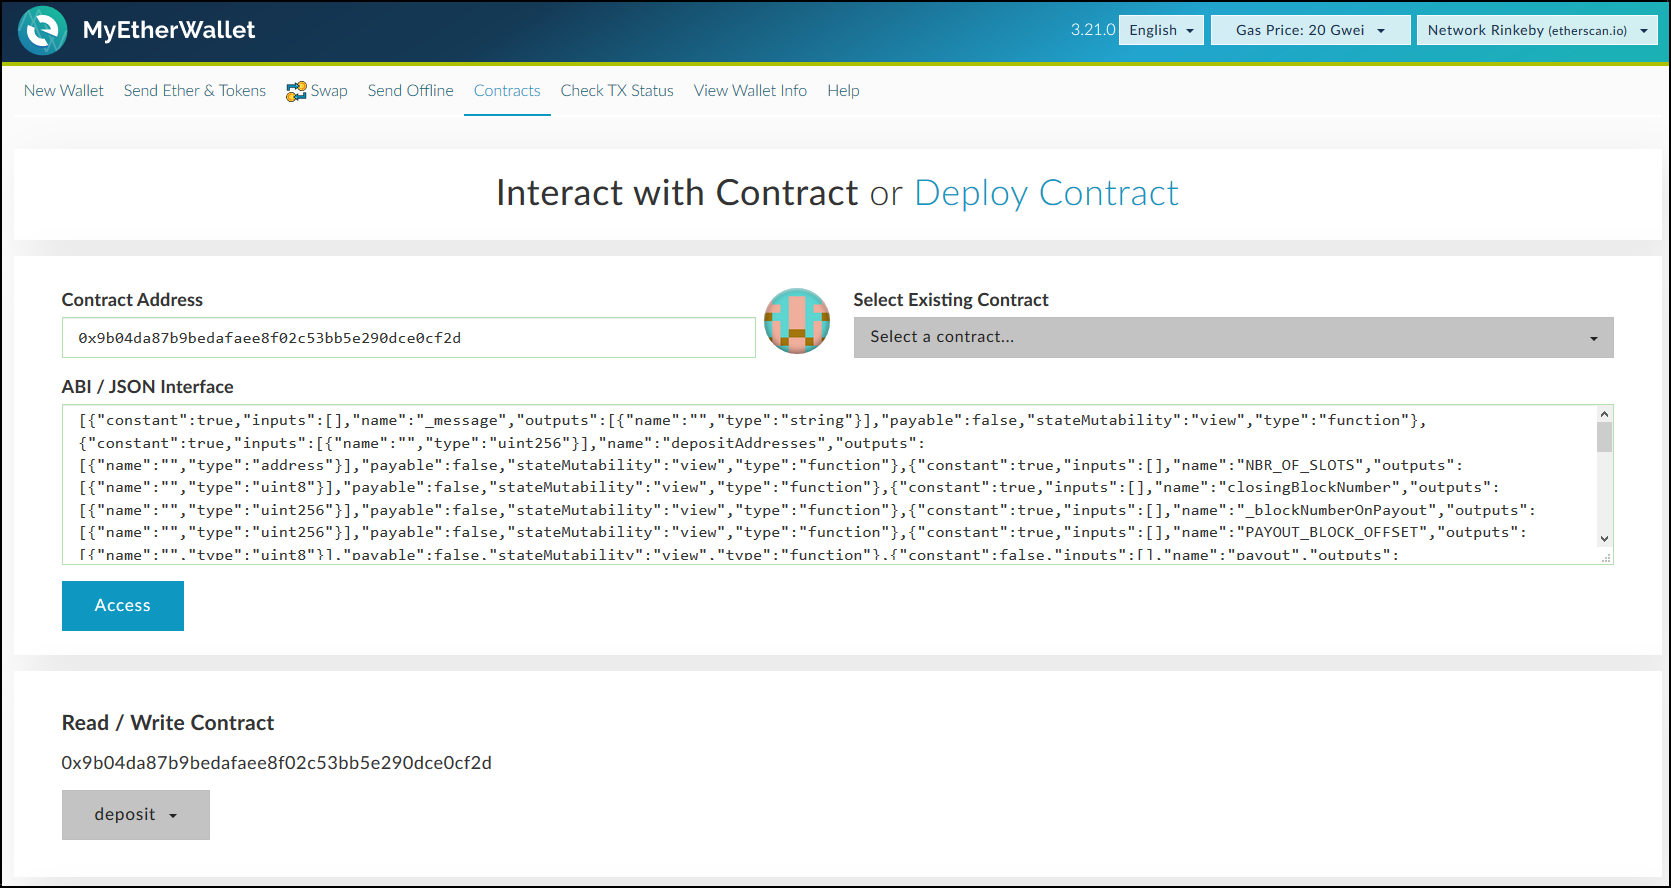
\includegraphics[width=1\linewidth]{Figures/eth_gui/ETH_wallet}
\decoRule
\caption{My Ether Wallet}
\label{fig:ETH_wallet}
\end{figure}

Nachdem der Nutzer diese wie in Abbildung \ref{fig:ETH_wallet} eingegeben hat kann er über eine Dropdown-Liste die gewünschte Funktion des Smart Contracts aufrufen.

\begin{figure}[H]
\centering
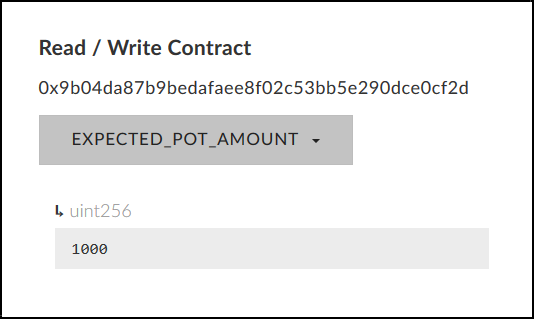
\includegraphics[scale=0.85]{Figures/eth_gui/ETH_wallet_expected_amount}
\decoRule
\caption{Aufruf der \code{EXPECTED POT AMOUNT} Funktion}
\label{fig:ETH_wallet_expected_amount}
\end{figure}

Abbildung \ref{fig:ETH_wallet_expected_amount} zeigt den Aufruf der Funktion auf, die zurückgibt, welchen Geldbetrag der Smart Contract vom Spieler erwartet. Da es sich lediglich um einen lesenden Zugriff handelt, wird keine Transaktion ans Netzwerk gesendet, beziehungsweise in die Blockchain geschrieben. Es fallen somit keine Transaktionskosten an.

\begin{figure}[H]
\centering
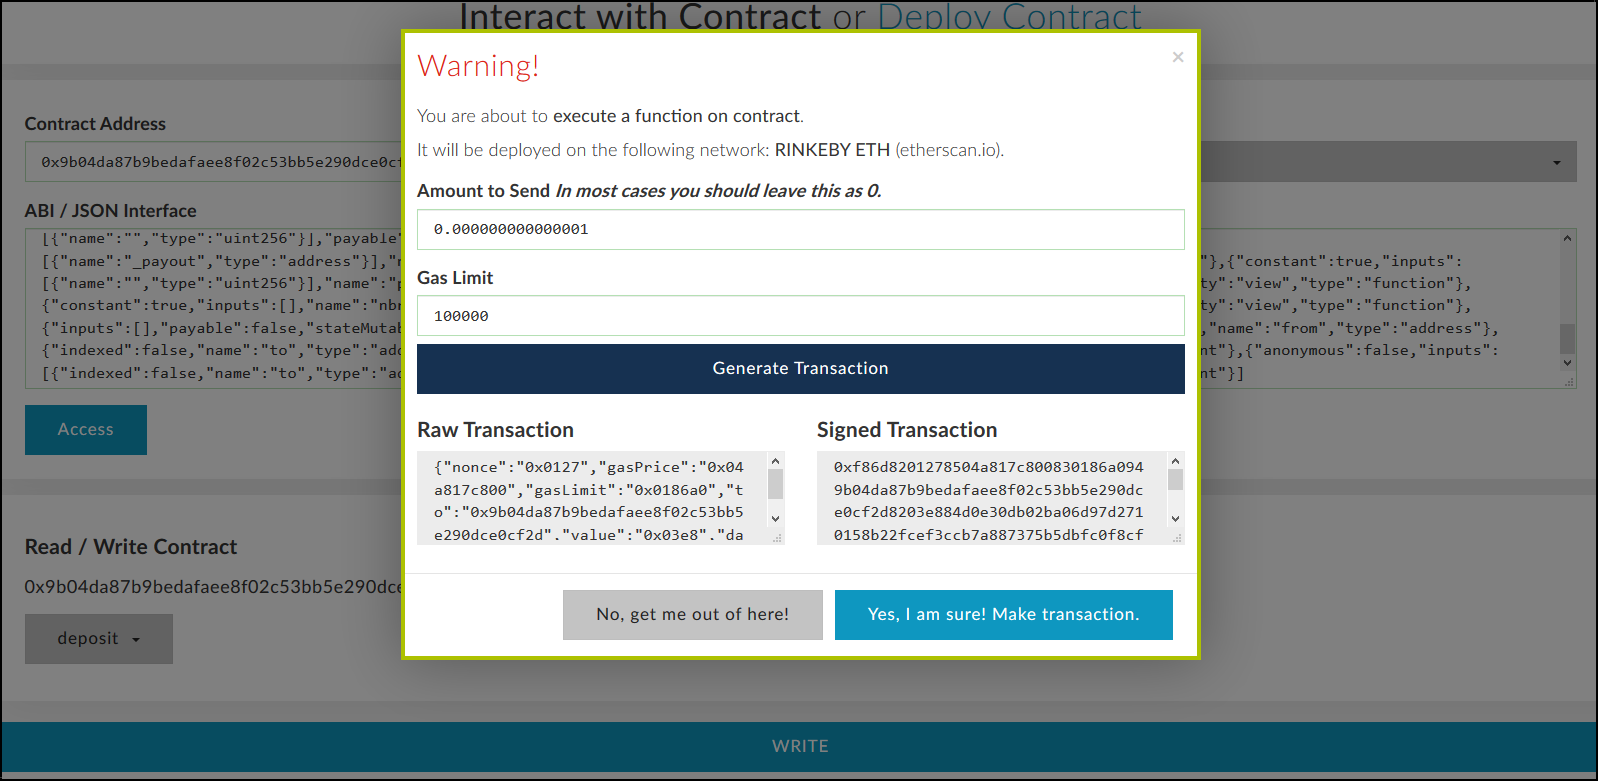
\includegraphics[width=1\linewidth]{Figures/eth_gui/ETH_wallet_deposit}
\decoRule
\caption{Aufruf der \code{deposit} Funktion}
\label{fig:ETH_wallet_deposit}
\end{figure}

Da der Nutzer nun nachgeprüft hat, dass der Smart Contract wirklich Zahlungen von 1000 WEI erwartet, kann er die \code{depsoit} Funktion mit diesem Betrag aufrufen.
Die Wallet Webseite erwartet den Betrag in der Einheit Ether. Die geforderten 1000 WEI entsprechen 0.000000000000001 Ether. Die Umrechnung kann der Spieler mittels eines Online Konverters\footnote{\url{https://etherconverter.online/}} durchführen.
Nun muss die erstellte Transaktion nur noch signiert werden. Der Nutzer kann der Webseite dazu seinen privaten Schlüssel mitteilen oder die Signierung eigenständig durch ein sogenanntes Hardware Wallet durchführen. Die Herausgabe seines privaten Schlüssels an eine Webseite ist aus sicherheitstechnischer Sicht keine gute Praktik. Sollte der Webseitenbetreiber böse Absichten haben oder die Webseite gehackt werden, führt dies zum Verlust des durch den Schlüssel kontrollierten Geldes. Eine sichere Variante ist die Verwendung eines Hardware Wallets. Dieses speichert alle privaten Schlüssel und führt die Signatur eigenständig durch. Der verwendete private Schlüssel verlässt somit niemals das Gerät. 

\begin{figure}[H]
\centering
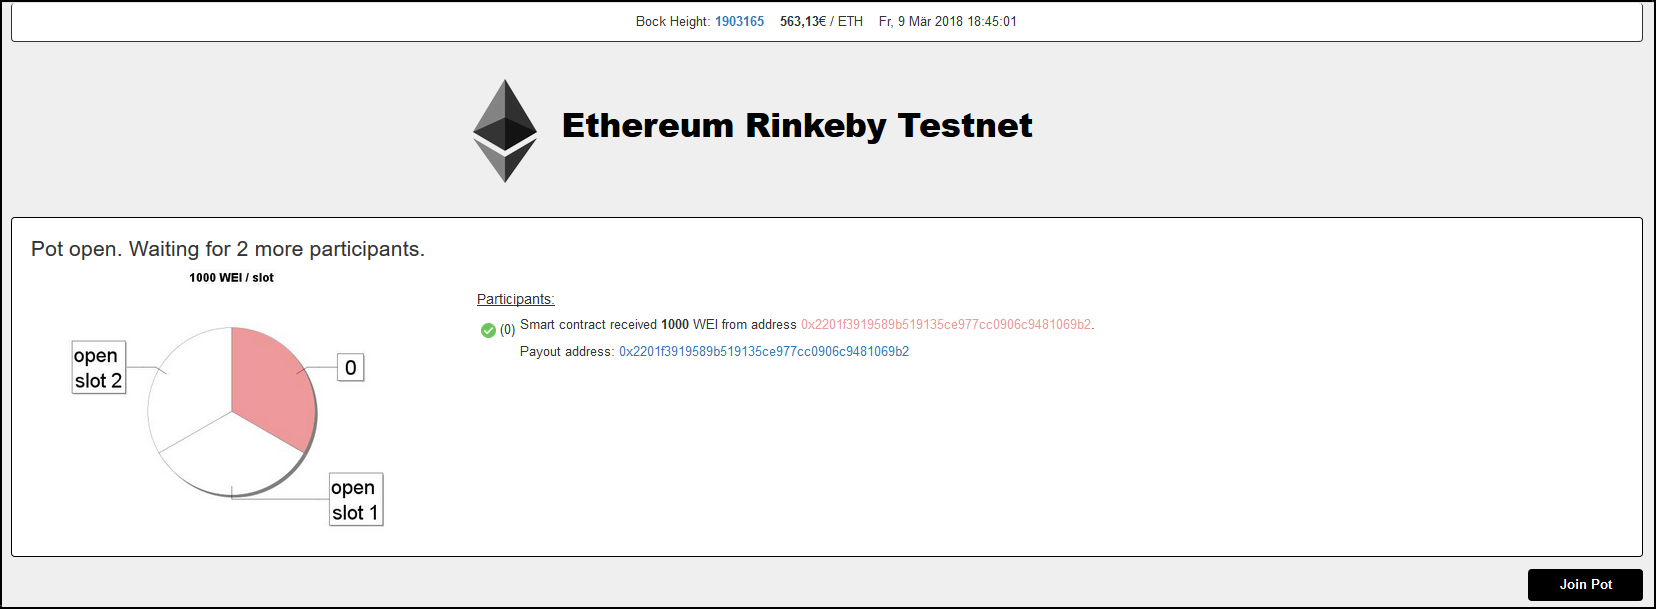
\includegraphics[width=1\linewidth]{Figures/eth_gui/ETH_pot_1}
\decoRule
\caption{Eingang der ersten Zahlung}
\label{fig:ETH_pot_1}
\end{figure}

Abbildung \ref{fig:ETH_pot_1} visualisiert den Zustand des Smart Contracts nachdem die erste Einzahlungstransaktion in die Blockchain aufgenommen wurde.

\begin{figure}[H]
\centering
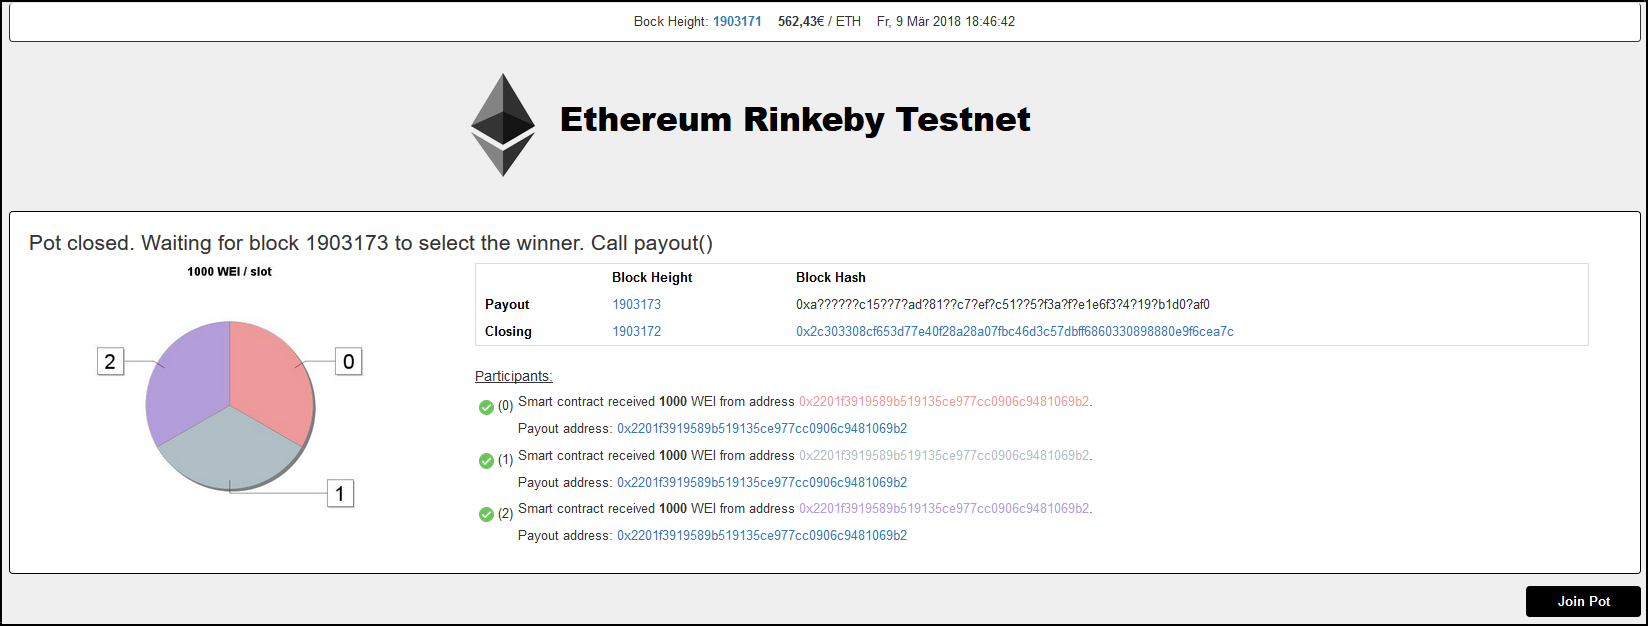
\includegraphics[width=1\linewidth]{Figures/eth_gui/ETH_pot_closed}
\decoRule
\caption{Topf geschlossen}
\label{fig:ETH_pot_closed}
\end{figure}

Abbildung \ref{fig:ETH_pot_closed} visualisiert den Zustand des Smart Contracts nachdem die letzte Einzahlungstransaktion in die Blockchain aufgenommen wurde. Der Smart Contract hat den Topf geschlossen und wartet nun, dass einer der Spieler die \code{payout} Funktion aufruft.

\begin{figure}[H]
\centering
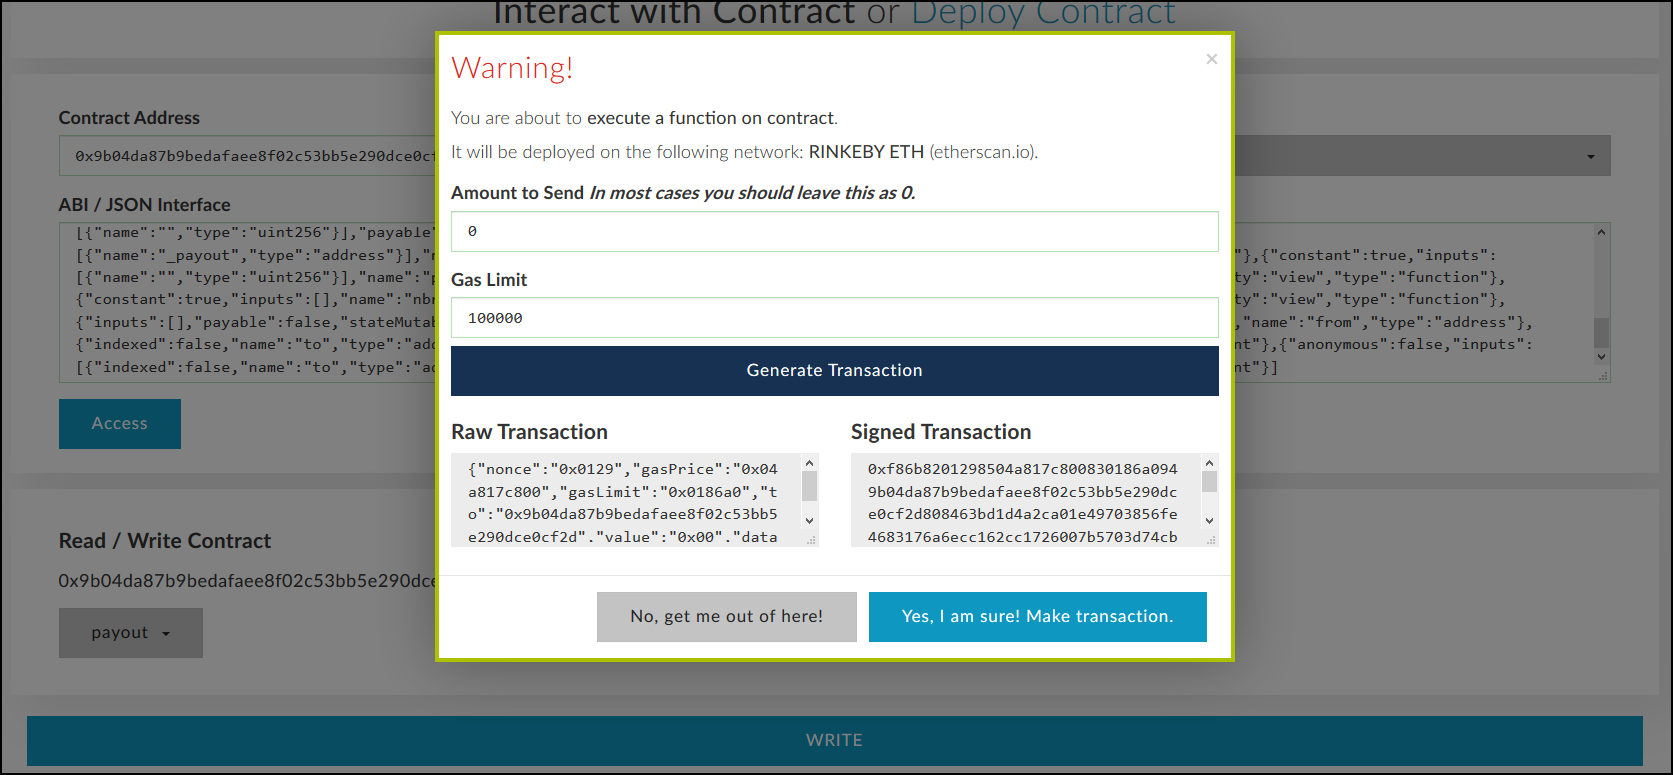
\includegraphics[width=1\linewidth]{Figures/eth_gui/ETH_wallet_payout}
\decoRule
\caption{Aufruf der \code{payout} Funktion}
\label{fig:ETH_wallet_payout}
\end{figure}

In Abbildung \ref{fig:ETH_wallet_payout} ist gezeigt wie ein Spieler die  \code{payout} Funktion aufruft. Durch den Aufruf dieser Funktion wird der Gewinner ausgewählt, die Auszahlung getätigt und der Topf wieder geöffnet.

\begin{figure}[H]
\centering
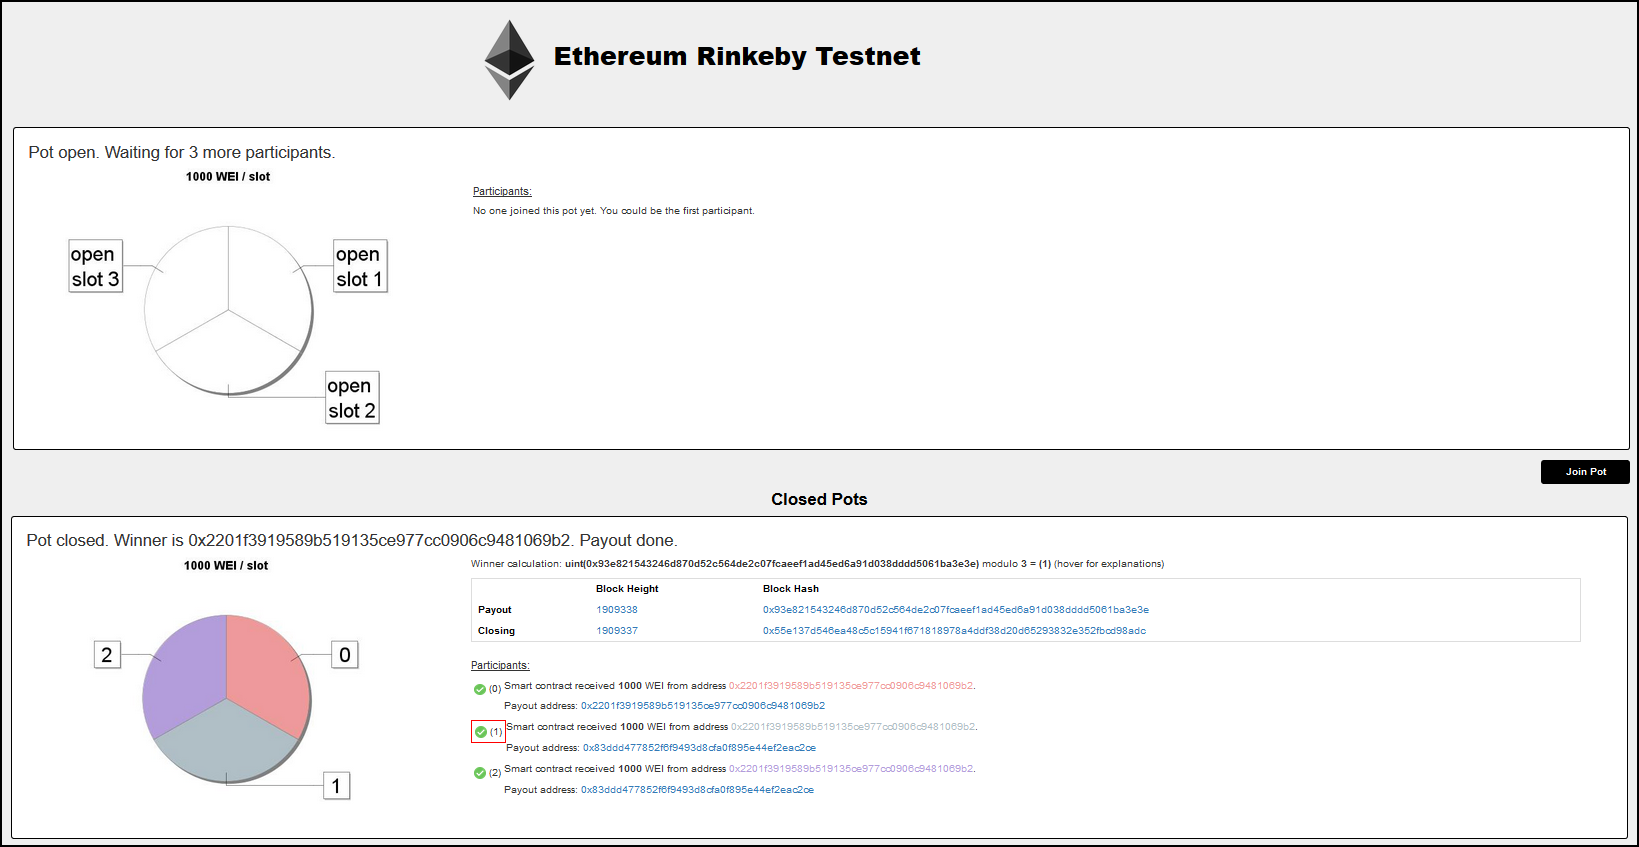
\includegraphics[width=1\linewidth]{Figures/eth_gui/ETH_pot_finished}
\decoRule
\caption{Gewinner ausgewählt}
\label{fig:ETH_pot_finished}
\end{figure}

Abbildung \ref{fig:ETH_pot_finished} zeigt den Gewinner des alten Topfs und den neu geöffneten Topf.